\documentclass[aspectratio=169,10pt]{beamer}

% ============================================================
%  Curso de Maestría — Métodos de Optimización
%  Clase 3 (complemento): tuning vs. tanteo -- cómo se ajustaron
%  T y step_size en los ejemplos manuales 1D
% ============================================================

\usepackage[utf8]{inputenc}
\usepackage[T1]{fontenc}
\usepackage{lmodern}
\usepackage[spanish]{babel}
\usepackage{amsmath,amssymb,amsthm}
\usepackage{graphicx}
\usepackage{booktabs}
\usepackage{xcolor}
\usepackage{listings}
\usepackage{tikz}

\graphicspath{{figs/}}

\usetheme{metropolis}
\metroset{block=fill, progressbar=frametitle, sectionpage=progressbar, numbering=fraction}

\definecolor{pygreen}{RGB}{0,128,0}
\definecolor{pyblue}{RGB}{0,0,180}
\definecolor{pygray}{RGB}{110,110,110}
\definecolor{codebg}{RGB}{245,245,245}

\lstdefinestyle{pythonstyle}{
  language=Python,
  backgroundcolor=\color{codebg},
  basicstyle=\ttfamily\scriptsize,
  keywordstyle=\color{pyblue}\bfseries,
  commentstyle=\color{pygreen}\itshape,
  stringstyle=\color{pygray},
  numbers=none,
  breaklines=true,
  showstringspaces=false,
  frame=single,
  rulecolor=\color{gray!40},
  xleftmargin=4pt,
  xrightmargin=4pt,
  aboveskip=6pt,
  belowskip=2pt,
}
\lstset{style=pythonstyle}

% --- notación abreviada ---
\newcommand{\R}{\mathbb{R}}
\newcommand{\grad}{\nabla}
\newcommand{\x}{\mathbf{x}}

\title{Métodos de Optimización}
\subtitle{Clase 3 (complemento): ¿tuning o tanteo?}
\author{[Nombre del profesor]}
\institute{Programa de Maestría, [Nombre de la universidad / programa]}
\date{Septiembre de 2026}

\begin{document}

% ---------------------------------------------------------------
\begin{frame}[plain]
  \maketitle
\end{frame}

\begin{frame}{De dónde sale esto}
  Los ejemplos manuales 1D de basin hopping, simulated annealing y PSO
  (material complementario de la Clase 3) sólo encuentran el mínimo
  global de forma confiable \textbf{después} de ajustar $T$, el
  \texttt{step\_size} y el peso de inercia $w$.
  \begin{alertblock}{La pregunta incómoda}
    Para llegar a esos valores corrí muchas combinaciones de
    hiperparámetros sobre varias semillas hasta quedarme con una que
    funcionara bien. \emph{¿Eso no es simplemente tanteo?}
  \end{alertblock}
  Respuesta corta: en parte sí, en parte no -- y la distinción importa
  mucho para usar estos métodos de forma responsable. Estas slides
  muestran el procedimiento completo, con datos.
\end{frame}

\begin{frame}{Dos cosas que se ven parecidas pero no lo son}
  \begin{columns}[T]
    \column{0.5\textwidth}
    \begin{block}{Tuning sistemático}
      \begin{itemize}
        \item Fijar una combinación de hiperparámetros.
        \item Correr \textbf{muchas semillas} distintas.
        \item Medir la \textbf{tasa de éxito} (¿qué fracción llegó al
          global?).
        \item Elegir la combinación con mejor tasa.
      \end{itemize}
    \end{block}
    \column{0.5\textwidth}
    \begin{block}{Cherry-picking (tanteo)}
      \begin{itemize}
        \item Correr con una semilla.
        \item Si no funciona, cambiar algo al azar.
        \item Repetir hasta que \textbf{una} corrida se vea bien.
        \item Publicar esa corrida como \emph{el resultado}.
      \end{itemize}
    \end{block}
  \end{columns}
  \vspace{0.3cm}
  \begin{exampleblock}{Lo que se hizo aquí}
    Un barrido de hiperparámetros (tuning sistemático) para elegir la
    \emph{región} de $(T,\text{step\_size})$; la semilla usada en cada
    figura (\texttt{seed=0}) fue la primera que se probó \textbf{dentro
    de esa región ya confiable} -- no una semilla especial elegida por
    su resultado.
  \end{exampleblock}
\end{frame}

\begin{frame}{El barrido real: basin hopping 1D}
  \begin{center}
    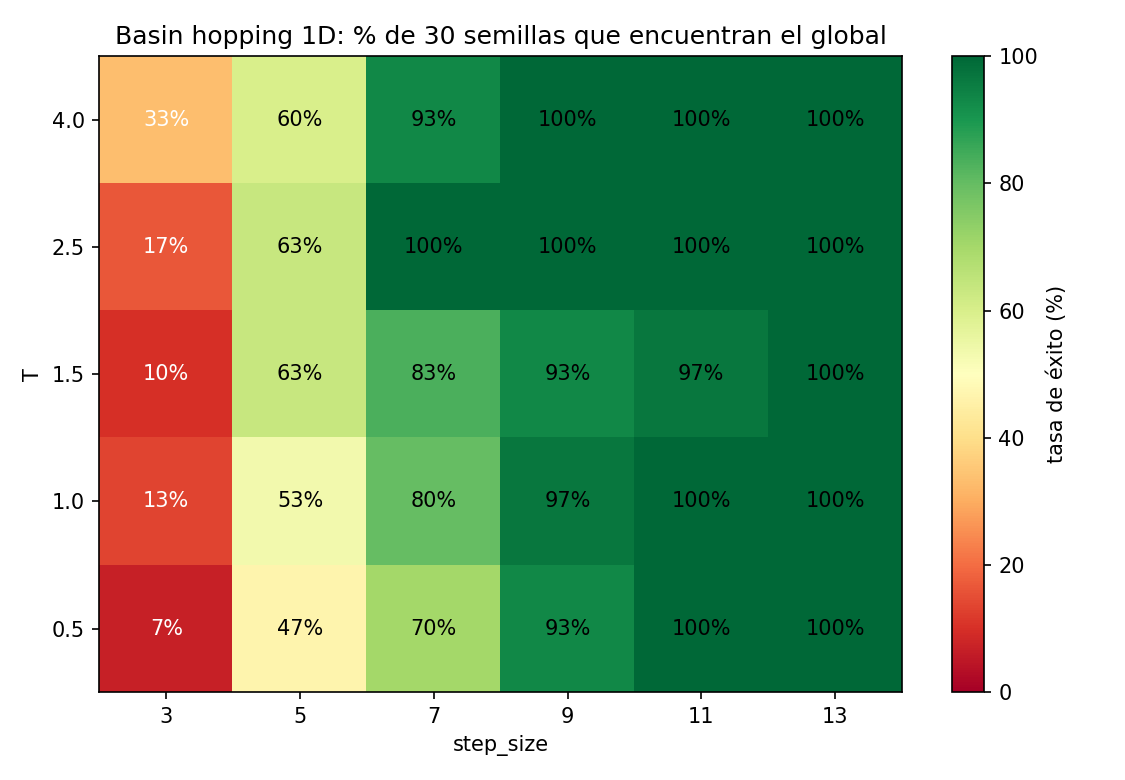
\includegraphics[height=6.3cm,keepaspectratio]{fig10_barrido_hiperparametros.png}
  \end{center}
\end{frame}

\begin{frame}[fragile]{Lo que dice el mapa de calor}
  \begin{itemize}
    \item \texttt{step\_size} importa \textbf{mucho más} que $T$ en
      este paisaje: con \texttt{step\_size}$\ge 9$ la tasa de éxito es
      $\ge 93\%$ para \textbf{cualquier} $T$ probado; con
      \texttt{step\_size}$=3$ nunca supera el 33\%, sin importar $T$.
    \item Esto tiene sentido: el mínimo global está a $\sim$15
      unidades del punto de arranque, y con saltos chicos casi nunca
      se cruza esa distancia en 30 iteraciones.
    \item \textbf{No hay una fórmula} que diga de antemano
      \emph{\texttt{step\_size}$=9$ es el correcto} -- eso solo se supo
      \emph{después} de correr el barrido.
  \end{itemize}
  \begin{block}{Con esos parámetros, ¿cualquier semilla funciona?}
\begin{lstlisting}
Basin hopping (step_size=9, T=1.5):      28/30 semillas (93%)
Simulated annealing (paso=3.5, T0=6):    28/30 semillas (93%)
Particle swarm (w: 0.9->0.4, N=20):      28/30 semillas (93%)
\end{lstlisting}
  \end{block}
  Sí: una vez encontrada la región correcta, la elección de semilla ya
  casi no importa. Eso es lo que hace \emph{tuning}, no
  \emph{cherry-picking}.
\end{frame}

\begin{frame}{El verdadero talón de Aquiles}
  \begin{alertblock}{El barrido necesitó algo que en la práctica no
    se tiene}
    Para medir \emph{tasa de éxito} hay que saber \textbf{dónde está el
    mínimo global} de antemano. En este ejemplo de clase lo sabemos
    (diseñamos la función). En un problema real de optimización se
    usa una metaheurística \textbf{precisamente porque no se conoce el
    paisaje} -- no hay vara de medir contra la cual calibrar $T$ o
    \texttt{step\_size}.
  \end{alertblock}
  \begin{center}
    \Large ¿Cómo se tunea algo cuando no se puede verificar si
    funcionó?
  \end{center}
\end{frame}

\begin{frame}{Qué se hace en la práctica, sin conocer la respuesta}
  \begin{itemize}
    \item \textbf{Diagnósticos relativos}: correr varias semillas y
      ver si \emph{convergen al mismo punto}. Coincidencia = buena
      señal (aunque no prueba que sea el global); resultados muy
      distintos entre semillas = señal de que faltan iteraciones o
      los hiperparámetros están mal.
    \item \textbf{Heurísticas basadas en la escala del problema}:
      \texttt{step\_size} como una fracción del rango de las
      variables; $T_0$ elegido para que la tasa de aceptación inicial
      sea $\sim$20--40\% (se estima con una muestra pequeña de
      $\Delta E$ típicos antes de correr todo el algoritmo).
    \item \textbf{Esquemas autoadaptativos}: ajustar
      \texttt{step\_size} solo, según la tasa de aceptación reciente
      (lo hace \texttt{scipy.optimize.basinhopping} internamente);
      mutación autoadaptativa en algoritmos genéticos; CMA-ES.
    \item \textbf{Aceptar la incertidumbre como parte del resultado}:
      reportar \emph{mejor de $N$ corridas independientes} en vez de
      \emph{la respuesta} -- lo que de hecho hacen la mayoría de los papers que
      usan estos métodos.
  \end{itemize}
\end{frame}

\begin{frame}{Síntesis}
  \begin{block}{}
    El ajuste de hiperparámetros que ven en los scripts 1D \textbf{sí}
    fue tuning sistemático (barrido + tasa de éxito sobre muchas
    semillas), no una semilla con suerte. Pero ese tuning se apoyó en
    conocer el mínimo global de antemano -- un lujo que un problema
    real casi nunca da.
  \end{block}
  \begin{exampleblock}{La lección honesta}
    Ninguna metaheurística viene con hiperparámetros \emph{correctos}
    de fábrica. Ajustarlos bien, sin hacer trampa, es en sí mismo
    parte del trabajo de optimizar -- y por eso en la práctica se
    combina con diagnósticos relativos, heurísticas de escala y
    reportar resultados de múltiples corridas en vez de una sola.
  \end{exampleblock}
  \small Hay un resultado teórico (Geman \& Geman, 1984) que garantiza
  convergencia al global con un enfriamiento \emph{logarítmico}
  $T_k=T_0/\log(k+2)$ -- pero es tan lento que nadie lo usa en la
  práctica; es la prueba de que existe una solución \emph{perfecta} a este
  problema, solo que es inútil computacionalmente.
\end{frame}

\begin{frame}{Referencias}
  \footnotesize
  \begin{itemize}
    \item S. Geman, D. Geman. \emph{Stochastic Relaxation, Gibbs
      Distributions, and the Bayesian Restoration of Images}.
      IEEE Trans.\ Pattern Analysis and Machine Intelligence,
      6(6), 1984. (Convergencia garantizada de SA con enfriamiento
      logarítmico.)
    \item N. Hansen. \emph{The CMA Evolution Strategy: A Tutorial}.
      arXiv:1604.00772, 2016.
    \item M. Kochenderfer, T. Wheeler. \emph{Algorithms for
      Optimization}. MIT Press, 2019.
    \item Scripts de referencia: \texttt{scripts/07\_basin\_hopping\_1d.py},
      \texttt{08\_simulated\_annealing\_1d.py},
      \texttt{09\_particle\_swarm\_1d.py},
      \texttt{10\_barrido\_hiperparametros\_1d.py}.
  \end{itemize}
\end{frame}

\begin{frame}[standout]
  ¿Preguntas?
\end{frame}

\end{document}
